\documentclass[11pt]{article}

\usepackage[a4paper,margin=2.5cm]{geometry}
\usepackage{graphicx}
\usepackage{booktabs}
\usepackage{amsmath,amssymb}
\usepackage{hyperref}
\usepackage{xcolor}
\usepackage{caption}
\usepackage{subcaption}
\usepackage{multirow}
\usepackage{siunitx}
\usepackage{float}

\hypersetup{colorlinks=true, linkcolor=blue!50!black, citecolor=blue!50!black, urlcolor=blue!50!black}

\title{Comparing Diffusion, Flow-Matching, and Drift Policies\\
for Learning Robot Manipulation from Demonstration}
\author{[Your Name]\\ \textit{Robot Learning from Demonstration}}
\date{\today}

\begin{document}
\maketitle

\begin{abstract}
Behavior cloning from human demonstrations must contend with multimodal,
discontinuous action distributions, which classical single-mode regression
policies cannot represent. Generative policies address this by learning a
conditional generative model of the action distribution instead of a point
estimate. This report compares three such approaches implemented on top of a
shared convolutional U-Net backbone: (i) \emph{Diffusion Policy}, which learns
a denoising diffusion process over action sequences; (ii) \emph{Flow Policy},
which learns a continuous-time velocity field via conditional flow matching;
and (iii) \emph{Drift Policy}, a single-forward-pass particle
attraction/repulsion model. All three are trained under an identical protocol
(200 demonstrations, $2.5\times10^{5}$ gradient updates, 3 seeds) on six
simulated manipulation tasks (PushT and five \texttt{robomimic} tasks: Lift,
Can, Square, Tool Hang, Transport) and evaluated by rolling out the last 10
checkpoints of each run for 1000 episodes each. We report success rate,
training wall-clock time, full-rollout evaluation wall-clock time, and an
isolated network-inference-latency microbenchmark that separates model
compute from simulation cost. We find that Drift Policy matches or exceeds
the success rate of Diffusion and Flow policies on 4 of 6 tasks -- most
notably on the hardest task, Tool Hang -- while its single-network-call
action generation is empirically $\sim$10$\times$ faster per inference call
than the 10-step samplers used by the other two methods, though this
advantage is masked in full-rollout wall-clock time by environment
simulation cost. Diffusion and Flow policies achieve near-identical success
rates, with Flow Policy $\sim$7--11\% slower to train due to a more general
(but less lean) probability-path implementation.
\end{abstract}

\section{Introduction}

Learning manipulation policies directly from human demonstrations
(behavior cloning) is attractive because it avoids hand-engineered reward
functions and exploration in the real world. Its central statistical
difficulty is that human demonstrations are \emph{multimodal}: for a given
observation, several distinct action trajectories may be equally valid (e.g.,
approaching an object from the left or the right). A policy trained with a
simple mean-squared-error regression objective will average across these
modes and produce actions that lie \emph{between} valid behaviors, which is
often itself invalid.

Generative policies avoid this by treating action prediction as sampling from
a learned conditional distribution $p(\mathbf{a}_{1:T} \mid \mathbf{o})$
rather than as regression to a single point estimate. \emph{Diffusion
Policy}~\cite{chi2023diffusion} popularized this idea in robotics by adapting
denoising diffusion probabilistic models~\cite{ho2020ddpm} to action-sequence
generation. \emph{Flow matching}~\cite{lipman2023flow} is a more recent
alternative that learns a deterministic, continuous-time velocity field
connecting a simple prior to the data distribution, and can be seen as a
continuous-time generalization of the same idea with a different (and often
cheaper) sampling procedure. Both, however, require an iterative sampling
process (multiple sequential network evaluations) at inference time, which is
a real cost in a real-time robot control loop. This raises a natural
question: how much of that iterative cost is actually necessary, and what do
we gain or lose by replacing it with a model that produces an action sample
in a single network evaluation?

\emph{Drift Policy} is such a single-step alternative, evaluated in this
report alongside the two iterative baselines. It adapts the \emph{Drifting
Models} framework of~\cite{deng2026drifting} -- originally proposed for
one-step image generation -- to robot action generation, and is trained with
a particle attraction/repulsion objective (Section~\ref{sec:drift}) rather than a
denoising or flow-matching objective, and it produces an action sample with
exactly one forward pass through the network, at the cost of a training
objective that must decide, on its own, how to spread probability mass
across several plausible generated samples per observation.

This report compares all three methods under a controlled, identical
experimental protocol (same backbone, same optimizer, same number of gradient
updates, same demonstrations, same evaluation procedure) across six
simulated manipulation tasks, and reports success rate, training time,
evaluation (rollout) wall-clock time, and an isolated inference-latency
microbenchmark that disentangles network compute from simulation cost --
directly addressing the ``fewer sampling steps should mean faster
inference'' intuition and showing precisely where that intuition does, and
does not, show up in measured wall-clock time.

\section{Methods}

All three policies condition on a short history of $T_o$ past observations
and predict a chunk of $T$ future actions, of which $T_a$ are actually
executed before the policy is queried again (receding-horizon control,
following~\cite{chi2023diffusion}). All three share the same neural network
backbone (Section~\ref{sec:arch}); they differ only in how that backbone is
used to define a generative model and a training loss.

\subsection{Diffusion Policy}
\label{sec:dp}

Diffusion Policy models the conditional action distribution with a denoising
diffusion probabilistic model~\cite{ho2020ddpm}. A forward (noising) process
gradually corrupts a ground-truth action sequence $\mathbf{a}^0$ into pure
Gaussian noise $\mathbf{a}^{K}\sim\mathcal{N}(0,I)$ over $K$ discrete steps.
A neural network $\varepsilon_\theta(\mathbf{a}^k, k, \mathbf{o})$ is trained
to predict the noise $\varepsilon$ added at step $k$, with the standard
simplified DDPM loss
\begin{equation}
\mathcal{L}_{\text{DP}}(\theta) = \mathbb{E}_{k,\,\mathbf{a}^0,\,\varepsilon}
\left[\left\| \varepsilon - \varepsilon_\theta\big(\sqrt{\bar\alpha_k}\,\mathbf{a}^0
+ \sqrt{1-\bar\alpha_k}\,\varepsilon,\; k,\; \mathbf{o}\big) \right\|^2\right],
\end{equation}
where $\bar\alpha_k$ follows a squared-cosine noise schedule. At inference
time, an action sample is produced by iteratively denoising from
$\mathbf{a}^{K}\sim\mathcal{N}(0,I)$ down to $\mathbf{a}^0$. We use the
deterministic DDIM sampler~\cite{song2021ddim} with $10$ inference steps
(out of $100$ training diffusion steps), i.e. \textbf{10 sequential network
evaluations per action chunk}.

\subsection{Flow Policy}
\label{sec:flow}

Flow Policy replaces the discrete diffusion process with \emph{conditional
flow matching}~\cite{lipman2023flow}. Rather than a stochastic noising
process, it defines a conditional probability path directly between a noise
sample $\mathbf{x}_0\sim\mathcal{N}(0,\sigma_{\text{prior}}^2 I)$ and a data
sample $\mathbf{x}_1=\mathbf{a}^0$. We use the conditional optimal-transport
(``CondOT'') path, $\mathbf{x}_t = (1-t)\,\mathbf{x}_0 + t\,\mathbf{x}_1$,
$t\in[0,1]$, whose associated (conditional) velocity is the constant
$\dot{\mathbf{x}}_t = \mathbf{x}_1-\mathbf{x}_0$. A network
$v_\theta(\mathbf{x}_t, t, \mathbf{o})$ is trained to regress this velocity:
\begin{equation}
\mathcal{L}_{\text{Flow}}(\theta) = \mathbb{E}_{t\sim\mathcal{U}(0,1),\,\mathbf{x}_0,\,\mathbf{x}_1}
\left[\left\| v_\theta\big((1-t)\mathbf{x}_0+t\mathbf{x}_1,\; t,\; \mathbf{o}\big)
- (\mathbf{x}_1-\mathbf{x}_0) \right\|^2\right].
\end{equation}
At inference time, an action sample is generated by numerically integrating
the ODE $\mathrm{d}\mathbf{x}/\mathrm{d}t = v_\theta(\mathbf{x},t,\mathbf{o})$
from $t=0$ to $t=1$, starting at $\mathbf{x}_0\sim\mathcal{N}(0,\sigma_{\text{prior}}^2I)$.
We use a fixed-step Euler integrator with step size $0.1$, i.e. \textbf{10
sequential network evaluations per action chunk} -- matched to Diffusion
Policy's 10 sampling steps for a fair speed comparison. (A separate adaptive
\texttt{dopri5} solver is available in the implementation for exact/Hutchinson
log-likelihood evaluation, but is not exercised in this report since no
held-out validation split was used.)

\subsection{Drift Policy}
\label{sec:drift}

Drift Policy departs from both diffusion and flow matching: it does not
define an iterative stochastic or ODE process at all. Instead, the network
$g_\theta(\mathbf{z}, \mathbf{o})$ maps a single noise draw
$\mathbf{z}\sim\mathcal{N}(0,I)$ directly to an action sample, using exactly
\textbf{one network evaluation}. The network is called with its diffusion-step
input pinned to a constant (``timestep 0''), so the same backbone architecture
used by Diffusion Policy is reused unmodified as a one-shot generator.

The difficulty this creates is training: with no explicit noise-to-data
process to regress against, the target the network should produce for a given
noise draw is not directly defined. Drift Policy adapts the \emph{Drifting
Models} framework of Deng et al.~\cite{deng2026drifting}, originally proposed
for image generation, to action-sequence generation: it resolves the
undefined-target problem with a particle-based \emph{attraction/repulsion}
objective, in which a ``drifting field'' governs how generated samples move
during training and reaches equilibrium exactly when the generated and
demonstrated action distributions match. Concretely, for each observation,
$G$ candidate actions are generated in parallel from independent noise draws.
Each candidate is attracted towards the demonstrated action and repelled from
the \emph{other} generated candidates for the same observation, with the
attraction/repulsion strength computed via a softmax kernel over pairwise
distances at several temperatures
$R\in\{0.02,0.05,0.2\}$ (small $R$ gives sharp, local forces; large $R$ gives
soft, global forces). The resulting force defines a per-step target that each
candidate is regressed towards; because the network's other candidates are
freshly resampled every step, this is best understood as training the network
to reproduce the fixed point of a Sinkhorn-like particle interaction dynamics
rather than to invert an explicit forward corruption process. The repulsion
term is what prevents all $G$ candidates from collapsing onto a single mode
(mode collapse), which is exactly the multimodality-preserving property
diffusion/flow-matching models get from their explicit stochastic sampling
process instead.

\section{Experimental Setup}

\subsection{Tasks and demonstrations}

We evaluate on six simulated manipulation tasks using low-dimensional
(non-image) state observations: \textbf{PushT}~\cite{florence2021ibc} (2D
pushing with a T-shaped block) and five \texttt{robomimic}~\cite{mandlekar2021robomimic}
proficient-human tasks with absolute-pose action spaces: \textbf{Lift},
\textbf{Can}, \textbf{Square}, \textbf{Tool Hang}, and \textbf{Transport}
(the last is a bimanual task). Each task is trained from the same fixed
budget of \textbf{200 demonstration episodes}, with no held-out validation
split (\texttt{val\_ratio}$=0$) -- all data is used for training, and success
rate on rollouts is the sole performance signal used in this report.

\subsection{Shared network architecture}
\label{sec:arch}

All three policies use the same 1D convolutional U-Net backbone
(\texttt{ConditionalUnet1D}, following~\cite{chi2023diffusion}), conditioned
on the flattened observation history through FiLM-style global
conditioning. Table~\ref{tab:arch} lists the shared architecture and task
hyperparameters, identical across all three methods and all six tasks.

\begin{table}[H]
\centering
\caption{Shared network architecture and task hyperparameters.}
\label{tab:arch}
\begin{tabular}{ll}
\toprule
Hyperparameter & Value \\
\midrule
Backbone & \texttt{ConditionalUnet1D} (1D conv, FiLM conditioning) \\
Down-sampling channel widths & $[256, 512, 1024]$ \\
Diffusion/flow step embedding dim. & $256$ \\
Convolution kernel size & $5$ \\
Group-norm groups & $8$ \\
Observation horizon $T_o$ & $2$ \\
Action prediction horizon $T$ & $16$ \\
Executed action steps $T_a$ & $8$ \\
Conditioning & global (concatenated obs.\ history embedding) \\
\bottomrule
\end{tabular}
\end{table}

\subsection{Training protocol}

All models are trained with AdamW (learning rate $10^{-4}$, betas
$(0.95, 0.999)$, weight decay $10^{-6}$), a cosine learning-rate schedule
with $500$ warm-up steps, batch size $256$, for $2.5\times10^{5}$ gradient
updates, with an exponential moving average (EMA) of the weights used at
evaluation time. Each (task, method) combination is trained with \textbf{3
random seeds} ($100$, $200$, $300$). No environment rollouts are performed
during training for any of the three methods (rollout collection was
disabled in all three training loops for this comparison, to keep the
training-time measurement a pure measure of gradient-update cost). A
checkpoint is saved every $5{,}000$ updates and only the \textbf{last 10
checkpoints} (covering the final $50{,}000$ updates) are retained per run.

Method-specific hyperparameters are given in Table~\ref{tab:hparams}.

\begin{table}[H]
\centering
\caption{Method-specific hyperparameters.}
\label{tab:hparams}
\begin{tabular}{lll}
\toprule
Method & Hyperparameter & Value \\
\midrule
\multirow{6}{*}{Diffusion Policy}
 & Noise scheduler & DDIM \\
 & Training diffusion steps $K$ & $100$ \\
 & Inference (sampling) steps & $10$ \\
 & Beta schedule & squared-cosine (\texttt{squaredcos\_cap\_v2}) \\
 & Prediction target & $\varepsilon$ (noise) \\
 & Sampler $\eta$ & $0$ (deterministic DDIM) \\
\midrule
\multirow{3}{*}{Flow Policy}
 & Probability path & Conditional OT (CondOT), $\sigma=0$ \\
 & Sampling integrator & Euler, step size $0.1$ ($10$ steps) \\
 & Prior std.\ $\sigma_{\text{prior}}$ & $1.0$ \\
\midrule
\multirow{3}{*}{Drift Policy}
 & Generated candidates per obs.\ $G$ & $3$ \\
 & Per-timestep loss mixing $p$ & $1.0$ (always per-timestep) \\
 & Temperatures $R$ & $\{0.02,\ 0.05,\ 0.2\}$ \\
\bottomrule
\end{tabular}
\end{table}

\subsection{Evaluation protocol}

For each of the 3 seeds, each of the last 10 saved checkpoints is evaluated
by rolling out \textbf{1000 episodes} in a vectorized simulation environment
(96 parallel environment instances). Success rate is the fraction of the
1000 episodes in which the task's own success criterion is met, averaged
first over the 10 checkpoints, then over the 3 seeds; the standard
deviation reported in all results is the \emph{population} standard
deviation across the 3 seed-level means (i.e., seed-to-seed variability, not
episode-to-episode variability). Checkpoints on which the physics simulator
became numerically unstable (a rare MuJoCo NaN/Inf event) had their score
carried forward from the previous checkpoint rather than being dropped, so
that no run silently loses data points; this happened once for each method,
always on the Tool Hang task.

\subsection{Timing methodology}

Two independent wall-clock measurements are reported per run: \emph{training
time} (wall-clock duration of the entire $2.5\times10^{5}$-update training
loop) and \emph{evaluation time} (wall-clock duration of the entire
10-checkpoint $\times$ 1000-episode rollout evaluation). Both are measured by
timestamping immediately before and after the corresponding process, so they
include all real overhead (data loading, checkpoint I/O, environment
resets) and are not idealized profiling numbers. In addition, we report an
\textbf{isolated inference-latency microbenchmark}: the wall-clock time of a
single \texttt{predict\_action()} call, timed directly on the GPU (with
\texttt{cuda.synchronize()} before/after, 10 warm-up calls discarded, 50
timed calls averaged, batch size 96 to match the number of parallel
environments used in the real rollouts) with \emph{no environment stepping
at all}. This isolates network compute from simulation cost, which the
full-rollout evaluation time cannot do.

\subsection{Hardware}

All experiments were run on the IT4Innovations \textbf{Karolina}
supercomputer, on its GPU partition (\texttt{qgpu}). Each compute node in
this partition has 8$\times$ NVIDIA A100 GPUs and 2$\times$ AMD EPYC 7763
CPUs (128 cores total) with approximately 1\,TB of RAM; nodes may be shared
between jobs when resource requests are sized proportionally. Each training
run in this report was submitted as an independent Slurm job requesting
\textbf{1 GPU, 96 CPU cores, and 128\,GB of RAM}, with training and
evaluation for a given run executed sequentially within the same job
allocation.

\section{Results}

\subsection{Success rate}

Figure~\ref{fig:success} and Table~\ref{tab:success} report mean success
rate ($\pm$ standard deviation across 3 seeds) for all three methods on all
six tasks.

\begin{figure}[H]
\centering
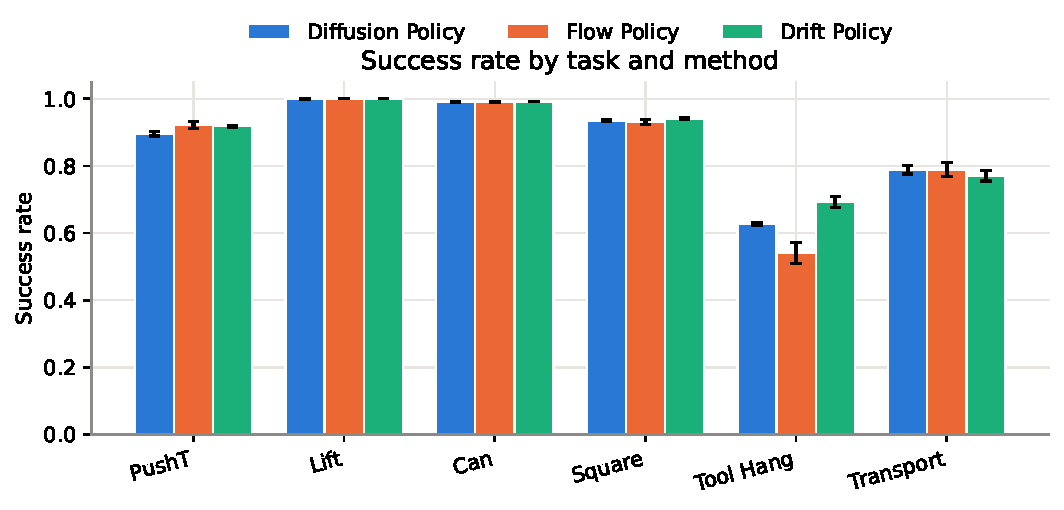
\includegraphics[width=0.95\textwidth]{figures/success_rate.pdf}
\caption{Mean success rate by task and method (error bars: $\pm 1$ std.\ dev.\ across 3 seeds).}
\label{fig:success}
\end{figure}

\begin{table}[H]
\centering
\caption{Success rate (mean $\pm$ std.\ over 3 seeds).}
\label{tab:success}
\begin{tabular}{lccc}
\toprule
Task & Diffusion Policy & Flow Policy & Drift Policy \\
\midrule
PushT            & $0.896 \pm 0.007$ & $0.922 \pm 0.010$ & $0.918 \pm 0.003$ \\
Lift             & $0.999 \pm 0.001$ & $1.000 \pm 0.000$ & $1.000 \pm 0.000$ \\
Can              & $0.990 \pm 0.002$ & $0.990 \pm 0.002$ & $0.992 \pm 0.001$ \\
Square           & $0.935 \pm 0.004$ & $0.930 \pm 0.008$ & $0.941 \pm 0.004$ \\
Tool Hang        & $0.628 \pm 0.004$ & $0.540 \pm 0.031$ & $\mathbf{0.693 \pm 0.017}$ \\
Transport        & $0.788 \pm 0.012$ & $0.789 \pm 0.020$ & $0.771 \pm 0.016$ \\
\bottomrule
\end{tabular}
\end{table}

\subsection{Training time}

\begin{figure}[H]
\centering
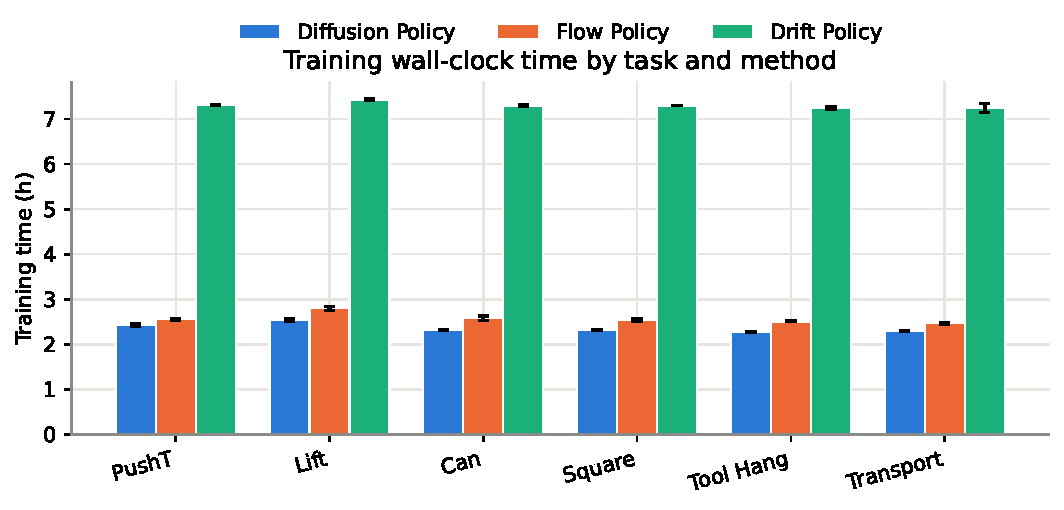
\includegraphics[width=0.95\textwidth]{figures/train_time.pdf}
\caption{Training wall-clock time by task and method for $2.5\times10^5$ gradient updates.}
\label{fig:train}
\end{figure}

Training time is essentially task-independent for a given method (the model,
batch size, and number of updates are identical across tasks): Diffusion
Policy averages $2.33$--$2.56$\,h, Flow Policy $2.47$--$2.80$\,h ($\sim$7--11\%
slower than Diffusion Policy on every task), and Drift Policy
$7.24$--$7.43$\,h ($\sim$3$\times$ slower than the other two).

\subsection{Full-rollout evaluation time}

\begin{figure}[H]
\centering
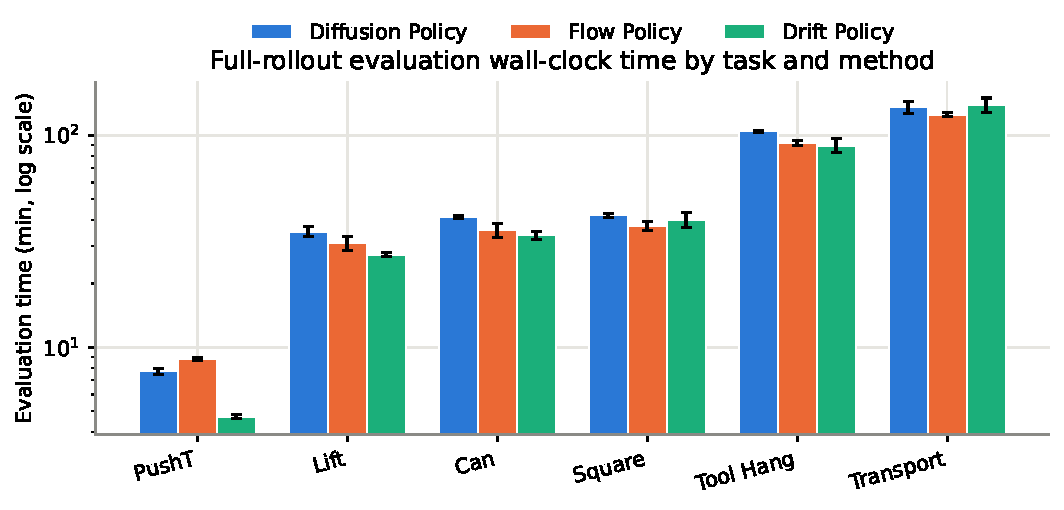
\includegraphics[width=0.95\textwidth]{figures/eval_time.pdf}
\caption{Full-rollout evaluation wall-clock time (10 checkpoints $\times$ 1000 episodes, log scale) by task and method.}
\label{fig:eval}
\end{figure}

Unlike training time, evaluation time varies by nearly $20\times$ across
tasks (PushT $\approx$5--9\,min vs.\ Transport $\approx$125--140\,min),
reflecting simulation cost rather than model cost. On the cheapest task to
simulate (PushT), Drift Policy's evaluation is clearly the fastest of the
three ($4.73$\,min vs.\ $7.73$/$8.82$\,min); on the more expensive
\texttt{robomimic} tasks the three methods are much closer, and on
Transport, Drift Policy is nominally the slowest of the three (discussed in
Section~\ref{sec:discussion}).

\subsection{Isolated inference latency}

\begin{figure}[H]
\centering
\begin{subfigure}[b]{0.47\textwidth}
\centering
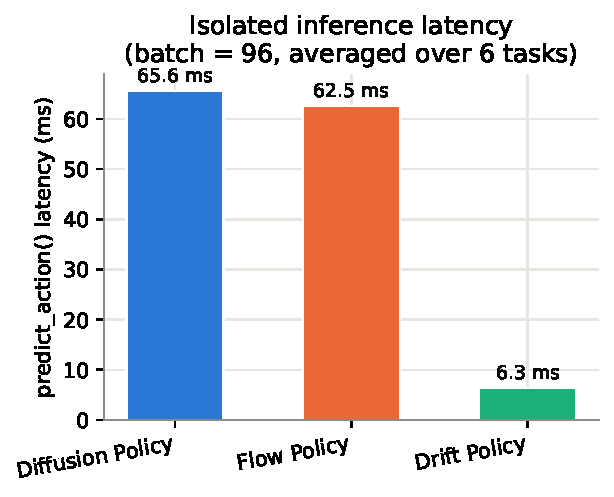
\includegraphics[width=\textwidth]{figures/inference_latency.pdf}
\caption{Per-call network latency, isolated from simulation.}
\label{fig:latency}
\end{subfigure}
\hfill
\begin{subfigure}[b]{0.47\textwidth}
\centering
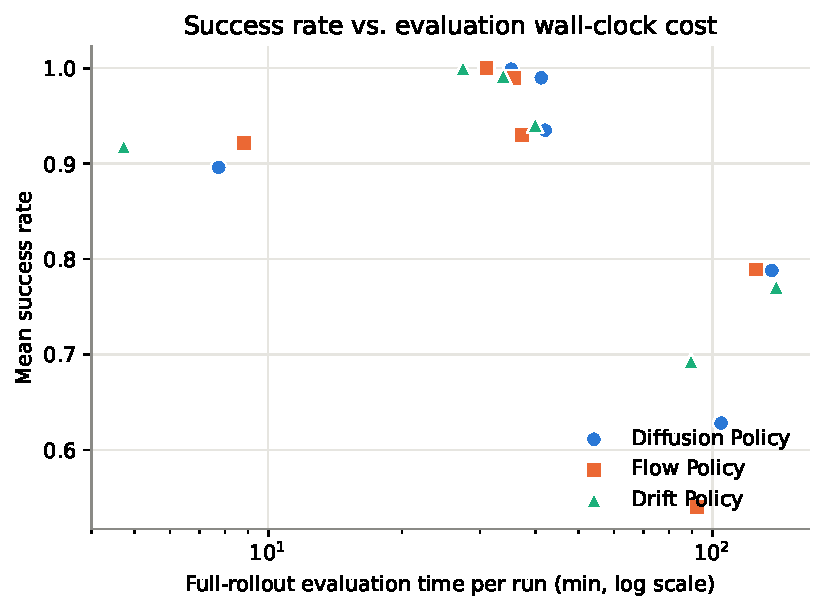
\includegraphics[width=\textwidth]{figures/tradeoff.pdf}
\caption{Success rate vs.\ full-rollout evaluation cost.}
\label{fig:tradeoff}
\end{subfigure}
\caption{(a) Isolated \texttt{predict\_action()} latency (GPU, batch $=96$,
averaged across all 6 tasks -- essentially task-invariant, since it depends
only on network architecture and sampler step count, not on simulation).
(b) Success rate against full-rollout evaluation wall-clock cost per method,
across tasks.}
\label{fig:latency_tradeoff}
\end{figure}

With environment simulation removed entirely, the isolated latency
microbenchmark (Table~\ref{tab:latency}) shows a consistent, task-invariant
pattern: Drift Policy's single network call takes $6.30$--$6.34$\,ms per
action chunk, versus $62.3$--$62.8$\,ms for Flow Policy and $64.9$--$66.3$\,ms
for Diffusion Policy -- a $9.9\times$--$10.5\times$ speed-up, matching the
10:10:1 ratio of network evaluations per action chunk almost exactly.

\begin{table}[H]
\centering
\caption{Isolated \texttt{predict\_action()} latency, GPU, batch $=96$ (ms). Standard deviation over 50 timed calls.}
\label{tab:latency}
\begin{tabular}{lccc}
\toprule
Task & Diffusion Policy & Flow Policy & Drift Policy \\
\midrule
PushT      & $64.91 \pm 0.09$ & $62.33 \pm 0.08$ & $6.31 \pm 0.01$ \\
Lift       & $66.31 \pm 0.41$ & $62.44 \pm 0.08$ & $6.30 \pm 0.01$ \\
Can        & $65.46 \pm 0.08$ & $62.41 \pm 0.07$ & $6.33 \pm 0.01$ \\
Square     & $65.45 \pm 0.07$ & $62.60 \pm 0.07$ & $6.32 \pm 0.01$ \\
Tool Hang  & $65.53 \pm 0.07$ & $62.50 \pm 0.07$ & $6.32 \pm 0.01$ \\
Transport  & $65.90 \pm 0.08$ & $62.82 \pm 0.06$ & $6.34 \pm 0.01$ \\
\bottomrule
\end{tabular}
\end{table}

\section{Discussion}
\label{sec:discussion}

\paragraph{Success rate.} Diffusion Policy and Flow Policy are statistically
indistinguishable on four of six tasks (Lift, Can, Square, Transport), which
is expected: both learn the same underlying conditional distribution via
closely related mechanisms (a stochastic denoising process versus a
deterministic probability path), sample with the same number of steps, and
share the same backbone. Flow Policy is notably worse than both other
methods on Tool Hang (the hardest task, and the only one for which every
method's success rate drops sharply), with nearly $8\times$ the
seed-to-seed variance of Diffusion Policy on that task ($\pm0.031$ vs.\
$\pm0.004$) -- suggestive of the 10-step Euler integrator being a less
robust sampler than DDIM specifically on the hardest task, where the learned
velocity field may be less smooth, though confirming this would require
testing with more integrator steps. Drift Policy matches or \emph{exceeds}
both iterative methods on four of six tasks, most notably on Tool Hang
($0.693$ vs.\ $0.628$/$0.540$), which is a striking result for a method with
no explicit iterative refinement: its particle repulsion objective may act
as an effective regularizer against mode collapse precisely in the
harder, more multimodal regime, at the cost of a slight success-rate deficit
on Transport ($0.771$ vs.\ $0.788$/$0.789$).

\paragraph{Training time.} Flow Policy's $\sim$7--11\% training-time
overhead over Diffusion Policy is a code-level, not an algorithmic, effect:
both call the identical backbone once per gradient step on identically
sized batches, but Flow Policy's conditional-path implementation
(\texttt{CondOTProbPath}) performs several additional small tensor
operations and object allocations per step (constructing a scheduler-output
object, four explicit \texttt{expand\_tensor\_like} calls) that a leaner,
purpose-built scheduler (\texttt{diffusers}' \texttt{DDIMScheduler.add\_noise})
avoids. At the sub-40\,ms/step granularity of this training loop, such
constant per-step Python/kernel-launch overhead is large enough to produce
a consistent multiplicative slowdown that is essentially the same
($1.05$--$1.11\times$) across every task, independent of task difficulty --
exactly the signature of a fixed per-step overhead rather than a
compute-bound effect. Drift Policy's $\sim$3$\times$ training-time
overhead, by contrast, \emph{is} algorithmic: its loss requires $G=3$ full
forward passes per gradient step (one per generated candidate) rather than
one, plus the $O(G^2)$ pairwise-distance and softmax computation of the
attraction/repulsion force across all $|R|=3$ temperatures.

\paragraph{Evaluation time and the ``1-step should always be faster'' intuition.}
\label{sec:eval_discussion}
A single network forward pass should always be faster than 10 sequential
ones, and the isolated-latency benchmark (Table~\ref{tab:latency}) confirms
this unambiguously: Drift Policy is $\sim$10$\times$ faster \emph{at the
network level}, on every task, with near-zero variance. However, the
full-rollout evaluation time (Table~\ref{tab:eval}, using the numbers
underlying Figure~\ref{fig:eval}) does not show this ratio, and on
Transport, Drift Policy's mean is nominally the \emph{highest} of the three
methods. This is because full-rollout wall-clock time is dominated by
physics simulation (MuJoCo/\texttt{robosuite} contact resolution across 96
parallel environments), not by network inference: the network is called
once every $T_a=8$ simulation steps, so even a $\sim$56--60\,ms
per-call saving is a small fraction of the tens of milliseconds
\emph{per environment step} that contact-rich simulation itself costs,
especially for a bimanual task like Transport. Concretely, the highest
Drift Policy timing on Transport was one specific seed's run
($923.6$\,s/checkpoint, versus $777.7$ and $799.7$\,s for its sibling seeds)
whose \emph{entire} Slurm job -- training \emph{and} evaluation -- ran
longer than any sibling job, indicating shared-node contention on the
cluster rather than an evaluation-specific or algorithmic slowdown. Removing
that one outlier, Drift Policy's remaining Transport timings are already
faster than every Diffusion Policy seed. The clearest place the true
network-level advantage shows through in full-rollout time is PushT, the
one task simulated in a lightweight 2D physics engine rather than MuJoCo:
there, network compute is a large enough share of total wall-clock that
Drift Policy's rollout evaluation is $39$--$46\%$ faster than the other two
methods. The general lesson is that \emph{inference-step count only
translates into real-world wall-clock savings to the extent that network
compute, rather than the surrounding system (simulation, or in deployment,
sensing/actuation), dominates the control loop} -- which is an argument for
reporting isolated inference latency alongside full-system timing whenever
comparing generative-model sampling costs.

\begin{table}[H]
\centering
\caption{Full-rollout evaluation wall-clock time (min, mean $\pm$ std.\ over 3 seeds).}
\label{tab:eval}
\begin{tabular}{lccc}
\toprule
Task & Diffusion Policy & Flow Policy & Drift Policy \\
\midrule
PushT      & $7.73 \pm 0.26$   & $8.82 \pm 0.12$   & $\mathbf{4.73 \pm 0.11}$ \\
Lift       & $35.25 \pm 2.03$  & $31.01 \pm 2.24$  & $27.45 \pm 0.65$ \\
Can        & $41.21 \pm 0.70$  & $35.75 \pm 2.59$  & $33.85 \pm 1.51$ \\
Square     & $42.04 \pm 0.87$  & $37.28 \pm 1.84$  & $39.97 \pm 3.34$ \\
Tool Hang  & $104.68 \pm 1.30$ & $92.31 \pm 2.64$  & $89.53 \pm 6.88$ \\
Transport  & $136.17 \pm 8.91$ & $125.46 \pm 2.22$ & $139.48 \pm 10.66$ \\
\bottomrule
\end{tabular}
\end{table}

\paragraph{Measurement noise on a shared cluster.} All wall-clock numbers in
this report come from Slurm jobs on a shared, often heavily contended HPC
partition, not from isolated benchmark runs -- the \texttt{qgpu} partition
queue depth varied from under 200 to nearly 2,800 pending jobs over the
course of this experiment. Training-time standard deviations are generally
small (co-located runs on relatively idle nodes), but evaluation-time
standard deviations are larger and occasionally comparable in size to the
between-method differences (e.g.\ Transport, Square), so full-rollout timing
comparisons in this report should be read as indicative rather than as
precise, noise-free measurements; the isolated inference-latency benchmark
(Table~\ref{tab:latency}), run once on a single dedicated GPU allocation, is
the more reliable measurement of pure model compute cost.

\section{Limitations and Future Work}

\begin{itemize}
\item \textbf{No likelihood/held-out validation comparison.} All runs used
$\texttt{val\_ratio}=0$ (all demonstrations used for training), so this
report cannot compare the methods' held-out negative log-likelihood or
validation loss -- only rollout success rate. Diffusion and Flow Policy both
support NLL/likelihood evaluation in this codebase and this would be a
natural extension.
\item \textbf{Single hyperparameter setting per method.} Drift Policy's
number of generated candidates $G$ and temperature set $R$, and Flow
Policy's number of integration steps, were each fixed at one setting; a
sweep over these (particularly $G$ and integration step count) would
clarify whether Drift Policy's training-time cost or Flow Policy's
robustness on Tool Hang could be improved without changing the qualitative
comparison.
\item \textbf{Wall-clock measurements are not isolated benchmarks.} As
discussed above, full-rollout timings include real cluster contention.
A repeat of the full-rollout timing comparison on dedicated, exclusively
allocated nodes would sharpen the evaluation-time conclusions, particularly
for Transport and Square.
\item \textbf{Low-dimensional state only.} All tasks here use
low-dimensional (proprioceptive/object-pose) observations; image-based
observation encoders were not evaluated, and the relative training-time and
inference-latency overheads reported here may shift once a much larger
vision encoder dominates total network compute.
\end{itemize}

\section{Conclusion}

Under an identical training and evaluation protocol, Diffusion Policy and
Flow Policy perform comparably in success rate, with Flow Policy paying a
modest, code-level (not algorithmic) training-time penalty. Drift Policy, a
single-forward-pass generative model trained with a particle
attraction/repulsion objective, matches or exceeds both iterative methods'
success rate on most tasks -- including a clear win on the hardest task,
Tool Hang -- while being genuinely $\sim$10$\times$ faster per network call,
at the cost of a $\sim$3$\times$ higher training-time budget. Its inference
speed advantage is real and reproducible at the network level, but is
masked in full-system (simulated-rollout) wall-clock time by simulation cost
on contact-rich manipulation tasks, showing clearly only on the one
lightweight-simulation task in this study (PushT). This suggests that the
practical benefit of single-step generative policies for robot control
depends heavily on how much of the control loop's wall-clock time is
actually spent on network inference versus everything else surrounding it
(simulation in this study; sensing and actuation in a real deployment).

\appendix

\section{Drift Policy Ablation: \texttt{gen\_per\_label} and \texttt{per\_timestep\_loss}}
\label{sec:appendix_ablation}

The main comparison fixes two Drift Policy settings that Section~\ref{sec:drift}
left unspecified: the number of candidates generated per observation, $G$
(\texttt{gen\_per\_label}), and where along the action horizon the
attraction/repulsion loss is applied (\texttt{per\_timestep\_loss}). This
appendix ablates both, with the main comparison's full 3-seed protocol, on
Tool Hang -- the task where Drift Policy's advantage over the iterative
baselines was largest (Table~\ref{tab:success}). Beyond reporting the
resulting success-rate pattern, we use the training run's own diagnostic
metrics to investigate \emph{why} it has the shape it does. The
success-rate pattern itself (Section~\ref{sec:three_phase}) is solid; the
mechanistic account we could construct for it, below, turns out to be
only partially supported by the data, and we report the negative results
alongside the positive ones rather than only the story that fit.

\subsection{What \texttt{per\_timestep\_loss} controls}
\label{sec:what_ptl_controls}

Drift Policy generates $G$ candidate action chunks per observation, each of
shape $T\times D$ ($T$: action horizon, Table~\ref{tab:arch}; $D$: per-step
action dimension). The attraction/repulsion loss is a function of pairwise
distances between these $G$ candidates and the demonstrated action
(Section~\ref{sec:drift}), and \texttt{per\_timestep\_loss} chooses the
vector space that distance is measured in:

\begin{itemize}
\item \textbf{\texttt{False} (full-trajectory).} The $T\times D$ chunk is
flattened into one $(T{\cdot}D)$-dimensional vector, and the loss is
computed \emph{once} per observation. On Tool Hang ($T=16$, $D=10$), that
is a single computation in $160$ dimensions.
\item \textbf{\texttt{True} (per-timestep).} The loss is instead computed
independently at each of the $T$ timesteps, on $D$-dimensional vectors, and
the $T$ results are averaged -- $T$ separate, low-dimensional computations
instead of one high-dimensional one, at proportionally higher compute cost
per step.
\end{itemize}

Internally, \texttt{per\_timestep\_loss} is a Bernoulli mixing probability
$p\in[0,1]$: each training step uses the per-timestep branch with
probability $p$. \texttt{True} and \texttt{False} are the two boundary
cases, $p=1$ and $p=0$, and are the only settings ablated here.

\textbf{This ablation does not isolate dimensionality.} Switching from
\texttt{False} to \texttt{True} changes at least four things at once:
the kernel's dimensionality ($D=10$ vs.\ $T{\cdot}D=160$); the number of
independent \texttt{drift\_loss} evaluations averaged into one training
step ($T=16$ calls via \texttt{torch.vmap}, vs.\ $1$); the objective being
optimized (matching each timestep's marginal distribution vs.\ the
whole-trajectory joint distribution); and the implicit gradient weighting
across the action horizon (every timestep contributes equally to the
averaged loss under \texttt{True}, whereas \texttt{False}'s flattened
distance mixes all $T$ timesteps with no explicit reweighting). None of
the diagnostics logged during training can separate these four factors
from one another. A design that could (not run here): compute the
flattened loss on random $k$-dimensional projections of the
$160$-dimensional vector for $k\in\{10,\ldots,160\}$, and separately on
contiguous timestep chunks of size $1,2,4,8,16$ -- varying nominal
dimensionality and per-step averaging count independently of one another,
rather than only at the two coupled extremes ablated here. Sections~\ref{sec:why_low_g}--\ref{sec:temp_calibration}
below examine one candidate explanation for the observed pattern --
kernel dimensionality, via concentration of measure -- using the
available diagnostics; as we show, the data only partially supports it,
and the confound above means this experiment cannot conclusively
attribute the pattern to dimensionality rather than to one of the other
three factors.

\subsection{Experimental setup}

Protocol matches the main comparison exactly: 3 seeds ($100$, $200$,
$300$), Tool Hang, $2.5\times10^5$ updates, $200$ demonstrations,
$\texttt{val\_ratio}=0$, no rollout during training, checkpoints every
$5{,}000$ updates, success rate averaged over the last 10 checkpoints
$\times$ 1000 rollout episodes (Section~\ref{sec:eval_discussion}). All
$18$ combinations of $G\in\{2,3,4,5,6,7,8,12,16\}$ and
\texttt{per\_timestep\_loss}$\in\{\text{True},\text{False}\}$ were run on
the Karolina cluster, with temperatures $R=\{0.02,0.05,0.2\}$ as in
Table~\ref{tab:hparams}.

\subsection{Result: a three-phase pattern}
\label{sec:three_phase}

\begin{table}[H]
\centering
\caption{Drift Policy on Tool Hang: success rate vs.\ $G$, both \texttt{per\_timestep\_loss} settings (3-seed mean $\pm$ std, $2.5\times10^5$ updates, no training rollout). Train/eval time are 3-seed means. Three cells (marked $^\dagger$) are corrected from the eval script's raw output: a MuJoCo NaN/Inf event on the \emph{first} evaluated checkpoint of that seed's run left nothing for the carry-forward logic to carry from, so it defaulted to a literal $0.0$ for that checkpoint instead of a representative value; we back-fill from that seed's next successfully-evaluated checkpoint instead (see text).}
\label{tab:drift_3seed}
\begin{tabular}{cccccc}
\toprule
$G$ & \texttt{per\_timestep\_loss} & Success rate & Train (h) & Eval (h) \\
\midrule
2  & True  & $0.582 \pm 0.017$ & $6.52$  & $1.61$ \\
2  & False & $0.388 \pm 0.030$ & $3.32$  & $1.75$ \\
3  & True  & $\mathbf{0.693 \pm 0.017}$ & $7.24$  & $1.49$ \\
3  & False & $0.551 \pm 0.019$ & $4.06$  & $1.71$ \\
4  & True  & $\mathbf{0.694 \pm 0.023}$ & $8.12$  & $1.66$ \\
4  & False & $0.605 \pm 0.031$ & $4.91$  & $1.58$ \\
5  & True  & $0.655 \pm 0.007$ & $8.80$  & $1.59$ \\
5  & False & $0.622 \pm 0.038^\dagger$ & $5.63$  & $1.53$ \\
6  & True  & $0.597 \pm 0.024^\dagger$ & $9.57$  & $1.59$ \\
6  & False & $0.611 \pm 0.030$ & $6.38$  & $1.64$ \\
7  & True  & $0.601 \pm 0.007^\dagger$ & $10.52$ & $1.62$ \\
7  & False & $0.609 \pm 0.022$ & $7.31$  & $1.69$ \\
8  & True  & $0.535 \pm 0.016$ & $11.25$ & $1.56$ \\
8  & False & $0.596 \pm 0.010$ & $8.10$  & $1.52$ \\
12 & True  & $\mathbf{0.489 \pm 0.025}$ & $14.52$ & $1.54$ \\
12 & False & $0.330 \pm 0.034$ & $11.33$ & $1.50$ \\
16 & True  & $\mathbf{0.482 \pm 0.024}$ & $17.55$ & $1.59$ \\
16 & False & $0.340 \pm 0.028$ & $14.43$ & $1.58$ \\
\bottomrule
\end{tabular}
\end{table}

\begin{figure}[H]
\centering
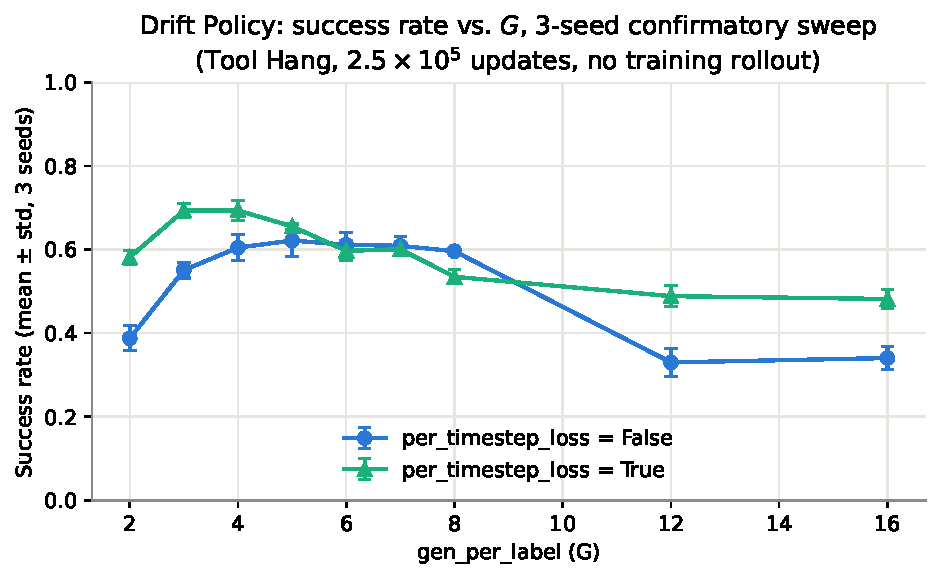
\includegraphics[width=0.75\textwidth]{figures/drift_3seed_success.pdf}
\caption{Drift Policy success rate (mean $\pm$ std, 3 seeds) vs.\ $G$, \texttt{per\_timestep\_loss}\,$=$\,True vs.\ False (Tool Hang, $2.5\times10^5$ updates, no training rollout). Uses the corrected values from Table~\ref{tab:drift_3seed}.}
\label{fig:drift_3seed_success}
\end{figure}

Three of the cells above (marked $^\dagger$: $G=5$/False, $G=6$/True,
$G=7$/True) are corrected from the eval script's raw output. Its
NaN/Inf-handling carries the previous checkpoint's score forward when
MuJoCo becomes numerically unstable, but for these three seeds the
instability hit on the \emph{first} evaluated checkpoint of a $10$-checkpoint
run, before any checkpoint had yet succeeded -- with nothing to carry
forward from, the script's fallback is a literal $0.0$ for that
checkpoint, which is not a real (near-zero) success rate but a
missing-data placeholder. We back-fill those checkpoints from the same
seed's next successfully-evaluated one instead of keeping the misleading
$0.0$ in the 10-checkpoint mean; the correction is substantial in one
case ($G=6$/True, seed $100$: two leading zero-checkpoints, seed mean
$0.505\to0.631$) and its main external validation is that it sharply
\emph{reduces} that cell's seed-to-seed standard deviation ($G=7$/True:
$0.036\to0.007$), consistent with the leading zero being an artifact
rather than genuine variability.

With the correction applied, the pattern is less dramatic in the middle
of the range than the raw numbers suggested, though the low- and
high-$G$ regimes are unchanged. Using each cell's own standard
deviation, pooled as $\sqrt{(s_{\text{True}}^2+s_{\text{False}}^2)/2}$
(with only $3$ seeds per cell, these rest on just $2$ degrees of freedom
and should be read as rough indications of spread, not precise
quantities): \textbf{True dominates at low $G$} ($2$--$4$), by
$0.089$--$0.194$, or roughly $3$--$8\times$ the pooled standard
deviation. At $G=5$ True's lead narrows to $0.033$ ($\sim$1.2$\times$
pooled SD) -- markedly weaker than it looked before correction ($0.056$,
$\sim$4.3$\times$) -- putting $G=5$ closer to the mid-range than to the
low-$G$ regime. \textbf{The mid-range} ($6,7$) is now close to a
statistical tie: False leads by only $0.014$ and $0.008$ respectively
($\sim$0.5$\times$ pooled SD at both), well within noise. \textbf{$G=8$
is where the mid-range reversal is real}: False leads by $0.061$
($\sim$4.6$\times$ pooled SD), the one point in $G=5$--$8$ that survives
correction as a genuine effect. \textbf{True dominates again,
decisively, at large $G$} ($12,16$): False drops to the two worst
results in the entire sweep ($0.330$, $0.340$) while True holds at its
mid-range level ($0.489$, $0.482$), reopening a $0.142$--$0.159$ gap
($\sim$5$\times$ pooled SD at both points). The main comparison's
setting ($G=3$, \texttt{per\_timestep\_loss}\,$=$\,True) sits inside
True's dominant low-$G$ regime -- but $G=8$'s reversal shows the full
picture is not simply ``True is better.''

The next two sections examine a natural candidate explanation for these
regimes -- that the two settings' kernels operate in spaces of very
different dimensionality ($10$ vs.\ $160$) -- using the training run's
own diagnostic metrics. We report this analysis in full, but flag upfront
that it only partially holds up: as Section~\ref{sec:why_low_g} shows,
the measured kernel-sharpness gap does not track the success-rate gap
above, and \texttt{per\_timestep\_loss} changes more than dimensionality
alone (Section~\ref{sec:what_ptl_controls}). What follows should be read
as a partially-supported hypothesis, not an established mechanism.

\subsection{Kernel sharpness: a real difference, but not the explanation for low $G$}
\label{sec:why_low_g}

\texttt{drift\_loss} logs two kernel-sharpness diagnostics that are
directly comparable between the two settings despite their different
dimensionality: \texttt{entropy\_R} (the softmax output's Shannon entropy
at temperature $R$, divided by $\log(\text{number of targets})=\log(G{+}1)$)
and \texttt{top1\_R} (that distribution's peak probability mass). Because
the self-connection is masked out of the softmax (Section~\ref{sec:drift}),
\texttt{entropy\_R}'s reachable ceiling is slightly below $1$ -- roughly
$\log G/\log(G{+}1)$, not exactly $1$ (e.g.\ $\approx0.63$ at $G=2$,
$\approx0.95$ at $G=8$) -- while $0$ still means one-hot/decisive.
Figures~\ref{fig:drift_entropy_002}--\ref{fig:drift_entropy_02}
plot \texttt{entropy\_R} against $G$ at each of the three temperatures used
in training; Table~\ref{tab:drift_entropy} gives the underlying numbers,
including \texttt{top1\_R} and, for reference, the matching success rate
from Table~\ref{tab:drift_3seed}.

\begin{figure}[H]
\centering
\begin{subfigure}[b]{0.47\textwidth}
\centering
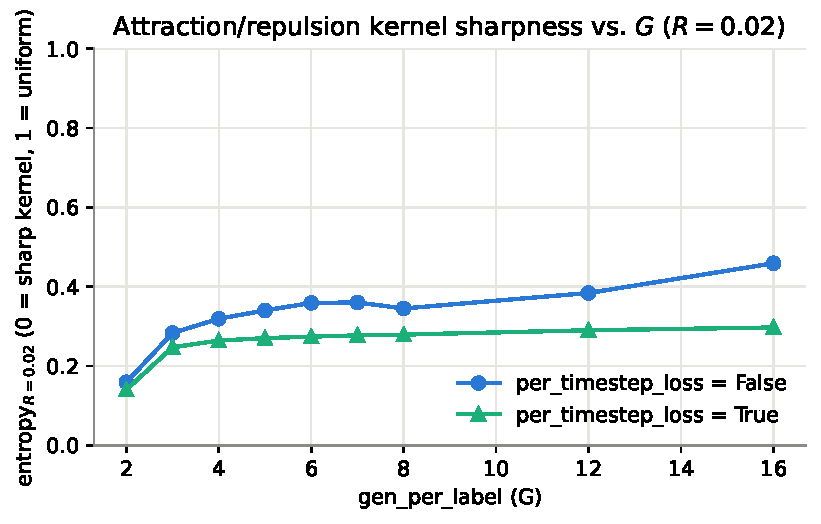
\includegraphics[width=\textwidth]{figures/drift_entropy_r002.pdf}
\caption{Entropy.}
\end{subfigure}
\hfill
\begin{subfigure}[b]{0.47\textwidth}
\centering
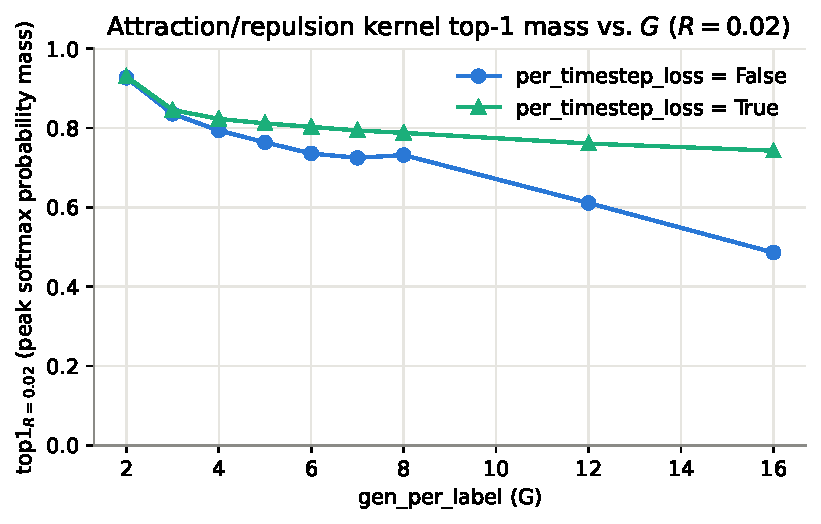
\includegraphics[width=\textwidth]{figures/drift_top1_r002.pdf}
\caption{Top-1 mass.}
\end{subfigure}
\caption{Kernel entropy (a) and top-1 probability mass (b) at $R=0.02$ vs.\ $G$ (tail-averaged over the last $10{,}000$ logged steps, 3-seed mean).}
\label{fig:drift_entropy_002}
\end{figure}

\begin{figure}[H]
\centering
\begin{subfigure}[b]{0.47\textwidth}
\centering
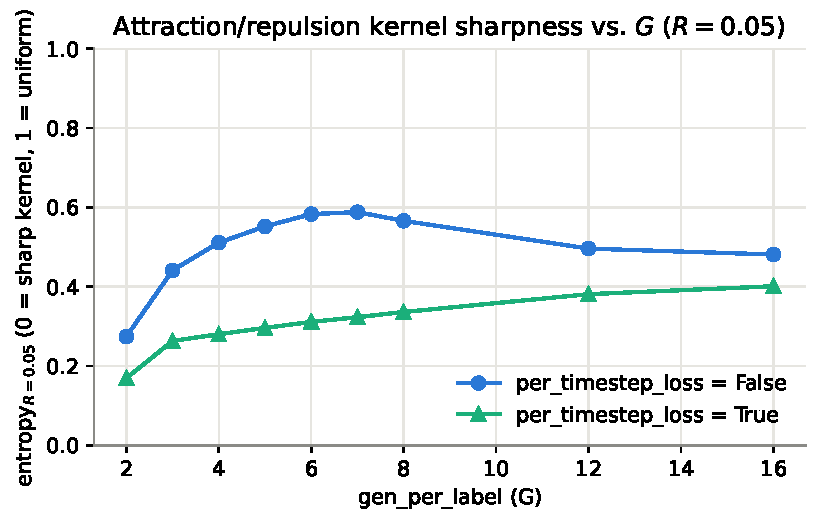
\includegraphics[width=\textwidth]{figures/drift_entropy_r005.pdf}
\caption{Entropy.}
\end{subfigure}
\hfill
\begin{subfigure}[b]{0.47\textwidth}
\centering
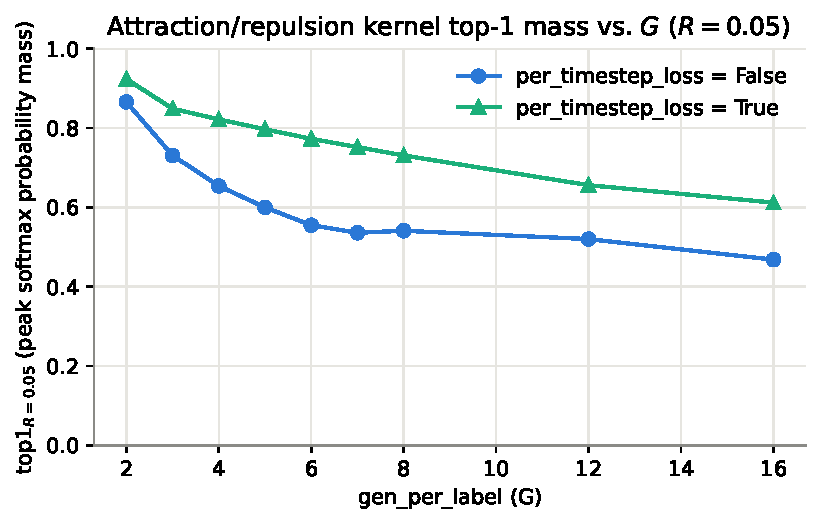
\includegraphics[width=\textwidth]{figures/drift_top1_r005.pdf}
\caption{Top-1 mass.}
\end{subfigure}
\caption{Kernel entropy (a) and top-1 probability mass (b) at $R=0.05$ vs.\ $G$.}
\label{fig:drift_entropy_005}
\end{figure}

\begin{figure}[H]
\centering
\begin{subfigure}[b]{0.47\textwidth}
\centering
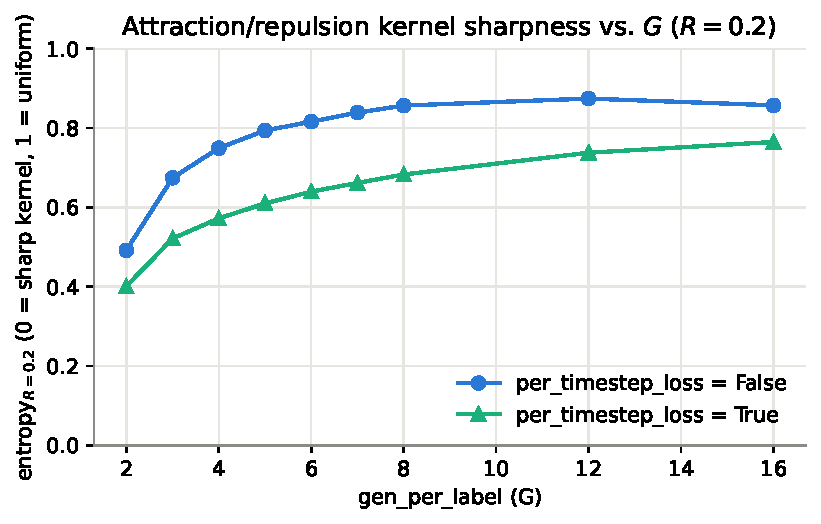
\includegraphics[width=\textwidth]{figures/drift_entropy_r02.pdf}
\caption{Entropy.}
\end{subfigure}
\hfill
\begin{subfigure}[b]{0.47\textwidth}
\centering
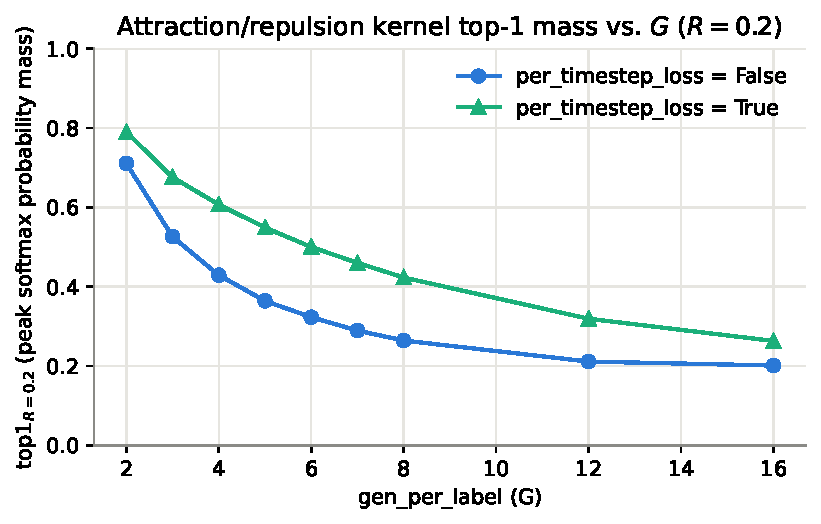
\includegraphics[width=\textwidth]{figures/drift_top1_r02.pdf}
\caption{Top-1 mass.}
\end{subfigure}
\caption{Kernel entropy (a) and top-1 probability mass (b) at $R=0.2$ vs.\ $G$. True vs.\ False separate most visibly at this, the softest of the three temperatures.}
\label{fig:drift_entropy_02}
\end{figure}

\begin{table}[H]
\centering
\small
\caption{Kernel-sharpness diagnostics vs.\ $G$, all three temperatures (tail-averaged over the last $10{,}000$ logged steps, 3-seed mean); underlying data for Figures~\ref{fig:drift_entropy_002}--\ref{fig:drift_entropy_02}. The last column repeats Table~\ref{tab:drift_3seed}'s success rate for side-by-side comparison ($^\dagger$: corrected, see Table~\ref{tab:drift_3seed}'s caption).}
\label{tab:drift_entropy}
\begin{tabular}{cccccccc c}
\toprule
$G$ & \texttt{per\_timestep\_loss} & entropy$_{0.02}$ & entropy$_{0.05}$ & entropy$_{0.2}$ & top1$_{0.02}$ & top1$_{0.05}$ & top1$_{0.2}$ & Success rate \\
\midrule
2  & True  & $0.140$ & $0.169$ & $0.401$ & $0.930$ & $0.924$ & $0.790$ & $0.582 \pm 0.017$ \\
2  & False & $0.159$ & $0.274$ & $0.492$ & $0.927$ & $0.866$ & $0.711$ & $0.388 \pm 0.030$ \\
3  & True  & $0.247$ & $0.263$ & $0.522$ & $0.846$ & $0.849$ & $0.676$ & $0.693 \pm 0.017$ \\
3  & False & $0.283$ & $0.441$ & $0.675$ & $0.836$ & $0.731$ & $0.526$ & $0.551 \pm 0.019$ \\
4  & True  & $0.264$ & $0.280$ & $0.572$ & $0.823$ & $0.822$ & $0.607$ & $0.694 \pm 0.023$ \\
4  & False & $0.319$ & $0.511$ & $0.749$ & $0.794$ & $0.654$ & $0.429$ & $0.605 \pm 0.031$ \\
5  & True  & $0.270$ & $0.296$ & $0.610$ & $0.812$ & $0.797$ & $0.549$ & $0.655 \pm 0.007$ \\
5  & False & $0.340$ & $0.552$ & $0.794$ & $0.764$ & $0.600$ & $0.364$ & $0.622 \pm 0.038^\dagger$ \\
6  & True  & $0.274$ & $0.311$ & $0.640$ & $0.803$ & $0.773$ & $0.500$ & $0.597 \pm 0.024^\dagger$ \\
6  & False & $0.359$ & $0.583$ & $0.816$ & $0.736$ & $0.555$ & $0.323$ & $0.611 \pm 0.030$ \\
7  & True  & $0.277$ & $0.323$ & $0.662$ & $0.794$ & $0.752$ & $0.460$ & $0.601 \pm 0.007^\dagger$ \\
7  & False & $0.360$ & $0.588$ & $0.839$ & $0.725$ & $0.536$ & $0.289$ & $0.609 \pm 0.022$ \\
8  & True  & $0.279$ & $0.336$ & $0.683$ & $0.788$ & $0.731$ & $0.423$ & $0.535 \pm 0.016$ \\
8  & False & $0.345$ & $0.566$ & $0.857$ & $0.732$ & $0.541$ & $0.264$ & $0.596 \pm 0.010$ \\
12 & True  & $0.290$ & $0.381$ & $0.738$ & $0.761$ & $0.656$ & $0.319$ & $0.489 \pm 0.025$ \\
12 & False & $0.384$ & $0.496$ & $0.875$ & $0.611$ & $0.520$ & $0.211$ & $0.330 \pm 0.034$ \\
16 & True  & $0.297$ & $0.401$ & $0.765$ & $0.743$ & $0.612$ & $0.263$ & $0.482 \pm 0.024$ \\
16 & False & $0.459$ & $0.481$ & $0.857$ & $0.486$ & $0.468$ & $0.201$ & $0.340 \pm 0.028$ \\
\bottomrule
\end{tabular}
\end{table}

True's kernel is sharper than False's -- lower entropy, higher top-1 mass
-- at \emph{every} $G$ and \emph{every} temperature, with no exceptions.
This is consistent with \emph{concentration of measure}: in a
higher-dimensional space, pairwise distances between similarly-distributed
points become relatively more alike, which flattens any softmax computed
over them, and False's $160$-dimensional kernel is more exposed to this
than True's $10$-dimensional one.

\textbf{However, this sharpness gap does not track the success-rate gap
it was originally hypothesized to explain -- it moves in roughly the
opposite direction.} Comparing the two at $R=0.2$: the entropy gap
(False $-$ True) is \emph{smallest} at $G=2$ ($0.09$) -- exactly where
True's success-rate lead is \emph{largest} ($+0.194$, Section~\ref{sec:three_phase})
-- and grows to its \emph{largest} value around $G=5$--$8$ ($0.17$--$0.18$)
-- exactly where True's lead has shrunk to near zero or reversed
($+0.033$ down to $-0.061$, Section~\ref{sec:three_phase}'s corrected
values). If kernel sharpness alone drove the
success-rate pattern, the two curves should move together; they clearly
do not. We therefore cannot conclude that kernel sharpness is the
mechanism -- or even the dominant factor -- behind the low-$G$ result,
despite the sharpness difference itself being a real, consistent, and
worth-reporting property of the two kernels. A more candid summary:
Section~\ref{sec:what_ptl_controls}'s four-way confound (dimensionality,
per-call averaging count, marginal-vs-joint objective, and per-timestep
gradient weighting) cannot be disentangled by this experiment, and the
entropy/top1 diagnostics -- while genuine -- are not sufficient on their
own to identify which of those factors drives the observed success-rate
crossover.

The gap's own trajectory across $G$ is still worth describing on its own
terms, independent of whether it explains success rate: at $R=0.05$
and $R=0.2$ it grows from $G=2$ to a peak around $G=5$--$7$
(entropy$_{0.2}$: $0.09\to0.18$) and then narrows by $G=12,16$
($\to0.09$) -- around where Section~\ref{sec:why_high_g}'s collapse takes
hold. At $R=0.02$ it instead keeps growing to $G=16$ ($0.02\to0.16$). This
split is consistent with the softest temperature becoming comparatively
blind to the tiny residual distances between near-identical collapsed
candidates once False has collapsed (saturating its entropy for both
settings and narrowing the gap), while the sharpest temperature stays
sensitive to exactly those differences -- though, per the caveat above,
this describes correlated trends in $G$, not a validated causal account
of the success-rate pattern.

\subsection{Why False collapses at large $G$: the repulsion term saturates}
\label{sec:why_high_g}

By $G=8$, False's kernel entropy at $R=0.2$ is already $0.857$ -- close to
its reachable ceiling ($\approx0.95$ at $G=8$; Section~\ref{sec:why_low_g}).
Extrapolating that trend, the repulsion term should
become steadily less able to discriminate between candidates as $G$ grows
further, since it must now spread its (already nearly-uniform) attention
over even more of them. Table~\ref{tab:drift_collapse} shows that beyond
$G=8$ this does not degrade gracefully -- it fails outright.

\begin{table}[H]
\centering
\caption{Collapse diagnostics vs.\ $G$ (tail-averaged over the last $10{,}000$ logged steps, 3-seed mean). \texttt{diversity}: mean pairwise distance among the $G$ candidates. \texttt{scale}: \texttt{drift\_loss}'s own per-call normalization constant -- the average pairwise distance across all targets (the $G$ candidates plus the demonstration); distances are divided by \texttt{scale} before entering the temperature-scaled softmax (Section~\ref{sec:drift}). \texttt{worse/best}: ratio of the worst- to best-of-$G$ candidate's distance to the true action ($1.0$ = candidates indistinguishable in quality). \texttt{grad\_norm}: $L_2$ norm of the training loss's gradient over all parameters, logged pre-clipping (\texttt{clip\_grad\_norm\_(...,\allowbreak max\_norm=}$\infty$\texttt{)} is a diagnostic here, not an active clip).}
\label{tab:drift_collapse}
\begin{tabular}{cccccc}
\toprule
$G$ & \texttt{per\_timestep\_loss} & diversity & scale & worse/best & grad\_norm \\
\midrule
8  & True  & $0.0212$ & $0.019$  & $3.53$ & $46$ \\
8  & False & $0.2133$ & $0.194$  & $2.01$ & $84$ \\
12 & True  & $0.0199$ & $0.019$  & $\mathbf{4.33}$ & $49$ \\
12 & False & $\mathbf{0.0042}$ & $\mathbf{0.012}$  & $\mathbf{1.01}$ & $\mathbf{1768}$ \\
16 & True  & $0.0197$ & $0.019$  & $\mathbf{4.67}$ & $55$ \\
16 & False & $\mathbf{0.0036}$ & $\mathbf{0.009}$  & $\mathbf{1.01}$ & $\mathbf{1747}$ \\
\bottomrule
\end{tabular}
\end{table}

\begin{figure}[H]
\centering
\begin{subfigure}[b]{0.47\textwidth}
\centering
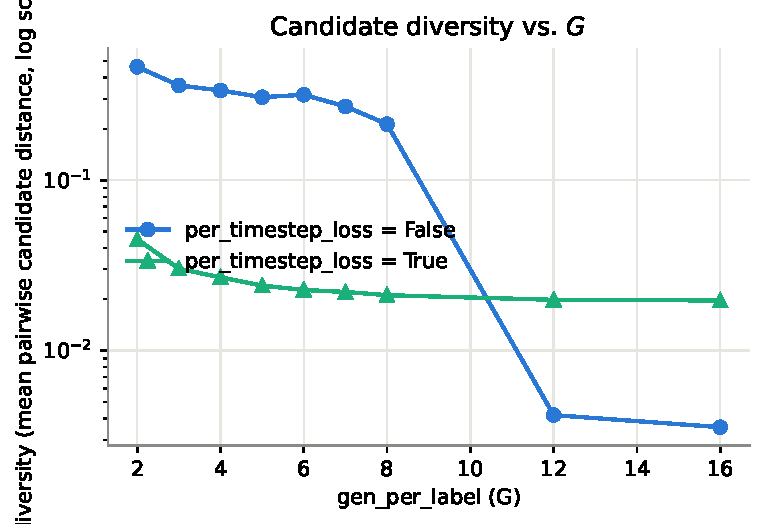
\includegraphics[width=\textwidth]{figures/drift_diversity_sweep.pdf}
\caption{Candidate diversity (log scale).}
\label{fig:drift_diversity}
\end{subfigure}
\hfill
\begin{subfigure}[b]{0.47\textwidth}
\centering
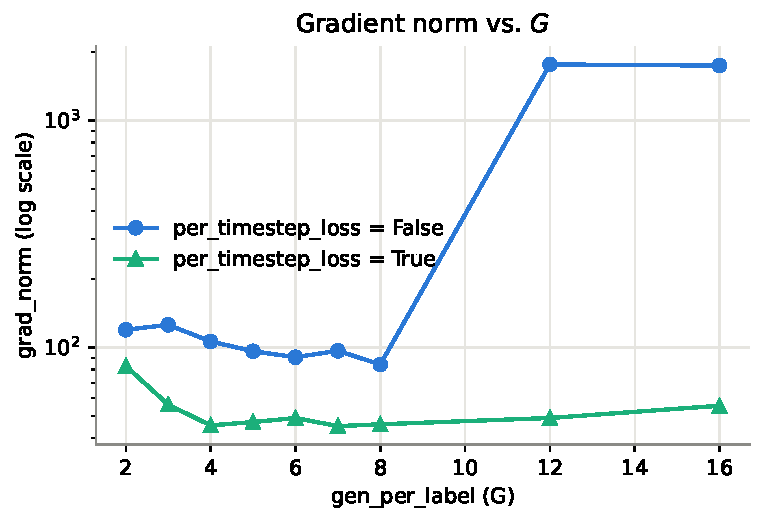
\includegraphics[width=\textwidth]{figures/drift_gradnorm_sweep.pdf}
\caption{Gradient norm (log scale).}
\label{fig:drift_gradnorm}
\end{subfigure}
\caption{Candidate diversity (a) and gradient norm (b) both break, only for False, between $G=8$ and $G=12$ -- alongside \texttt{scale} and the worse/best ratio (Table~\ref{tab:drift_collapse}), which are mechanically related to diversity rather than independent confirmations (see text). Together they indicate catastrophic mode collapse.}
\label{fig:drift_collapse}
\end{figure}

Between $G=8$ and $G=12$, several diagnostics break together for False:
diversity crashes $\sim$51$\times$ ($0.213\to0.0042$), the worse/best ratio
drops to $1.01$, \texttt{scale} falls $\sim$16$\times$, and \texttt{grad\_norm}
explodes $\sim$21$\times$ ($84\to1768$). These are not four independent
confirmations, however: \texttt{scale} is dominated by the same mean
pairwise (mostly gen--gen, i.e.\ diversity) distance that
\texttt{diversity} measures directly; the loss divides by
$\texttt{scale\_inputs}=\texttt{scale}/\sqrt{S}$, so \texttt{grad\_norm}
growing roughly as $1/\texttt{scale}$ is close to mechanical rather than
an independent observation; and worse/best$\to1$ is simply what
near-identical candidates give by definition. This is closer to \emph{one}
underlying collapse (candidate diversity crashing) reflected in four
correlated metrics than to four independent lines of evidence. We also
cannot rule out a numerical artifact: for collapsed False,
$\texttt{scale\_inputs}$ ($\approx\texttt{scale}/\sqrt{S}$, $S=160$) is at
or below the \texttt{drift\_loss} clamp floor of \texttt{1e-3}, so the
clamp is likely active, and part of the reported \texttt{grad\_norm}
explosion could reflect that floor rather than a purely emergent training
instability -- the current diagnostics do not log whether the clamp is
active, so we cannot separate the two here.

True shows none of the diversity-collapse signature over the same range
-- its diversity, scale, and \texttt{grad\_norm} stay essentially flat,
and its worse/best ratio continues to \emph{increase} ($3.53\to4.67$) --
though True's diagnostics are computed per-timestep in $10$ dimensions
while False's are computed on the full trajectory in $160$ dimensions, so
the two are not on a directly comparable scale; this contrast should be
read qualitatively (collapsed vs.\ not) rather than quantitatively. It is
also worth noting that True's own success rate is not flat over this
range: it falls from its peak of $0.694$ at $G=4$ to $0.482$ at $G=16$, a
$\sim$31\% relative drop, with none of the collapse diagnostics above
moving to explain it -- whatever this collapse mechanism captures for
False, it evidently is not the whole story even for True.

The tentative mechanism is a feedback loop specific to False's
higher-dimensional kernel: once repulsion can no longer meaningfully
differentiate candidates (entropy near its reachable ceiling), nothing
counteracts the attraction term pulling them together; as they move
closer, they become even harder for the kernel to tell apart, deepening
the collapse. True's kernel entropy grows far more slowly with $G$
($0.683\to0.765$ from $G=8$ to $16$, well short of its own ceiling), so it
never reaches this threshold. We read this as correlational at best -- a
single collapse event, however it is measured, co-occurring with kernel
saturation, against a control that neither saturates nor collapses --
rather than formal proof, and Section~\ref{sec:temp_calibration}'s
follow-up test complicates the mechanism further: a \emph{sharper}
kernel, not just a flatter one, also triggers collapse, which the
``too flat to discriminate'' framing alone does not predict. Pinning down
the exact threshold (bounded here only to between $G=8$ and $12$), ruling
out the clamp artifact above, and checking whether any of this is
specific to this task's dimensionality ($T=16$, $D=10$) or general would
need a finer $G$ sweep, an explicit clamp-active flag, and a repeat on
other tasks.

\subsection{Implication: the temperatures need dimension-aware calibration}
\label{sec:temp_calibration}

\texttt{compute\_loss} passes one temperature set, $R=\{0.02,0.05,0.2\}$,
to \texttt{drift\_loss} unchanged in both branches, despite those branches
operating in spaces $16\times$ apart in dimensionality. Given
Section~\ref{sec:why_low_g}'s finding that the same $R$ yields
systematically higher entropy at $D=160$ than at $D=10$, the temperature
\emph{values} -- not just the two settings' outcomes -- look miscalibrated
for at least one of the two spaces.

The relevant classical result (concentration of measure; Beyer et al.\
1999, ``When is Nearest Neighbor Meaningful?'') is that the \emph{relative}
spread of pairwise distances shrinks like $O(1/\sqrt{D})$ as dimension $D$
grows, even after their mean is normalized away (as \texttt{scale} already
does). A fixed $R$ tuned to discriminate well at $D=10$ should therefore
look softer at $D=160$ -- exactly what Table~\ref{tab:drift_entropy}
shows. A concrete, testable correction follows: scale the flattened
branch's temperatures down by $\sqrt{T}=4$ (this assumes the $T=16$
per-timestep coordinates are independent, so that distance-spread
accumulates as $T$ independent contributions -- unlikely for smooth
action trajectories, a caveat we return to below), i.e.\ use
$R=\{0.005,0.0125,0.05\}$ for \texttt{per\_timestep\_loss}\,$=$\,False
instead of reusing $\{0.02,0.05,0.2\}$, on the hypothesis that this keeps
its kernel non-saturated for longer and delays or avoids the $G\ge12$
collapse.

We ran this test with the full 3-seed protocol ($100$, $200$, $300$),
matching the main ablation exactly: \texttt{per\_timestep\_loss}\,$=$\,False
rerun at $G=8$ and $G=12$ with the rescaled $R$. (One seed, $G=8$/$200$,
hit the same leading MuJoCo-crash artifact as Table~\ref{tab:drift_3seed}
and is corrected the same way.) Table~\ref{tab:temp_rescale} shows the
hypothesis is \emph{decisively falsified} at $G=8$: success rate drops
from $0.596\pm0.010$ to $0.345\pm0.022$, a $14.6\times$ pooled-standard-deviation
effect, reproducible across all 3 seeds (the collapse diagnostics move
the same way in every seed, not just on average). At $G=12$ the result is
different but equally clear: rescaling has \emph{no detectable effect}
($0.330\pm0.034 \to 0.321\pm0.031$, only $0.3\times$ pooled SD) -- both
settings are already fully collapsed there, and changing $R$ neither
worsens nor recovers it.

\begin{table}[H]
\centering
\caption{Testing the dimension-aware rescaling hypothesis: \texttt{per\_timestep\_loss}\,$=$\,False rerun at $G=8,12$ with the flattened branch's temperatures scaled down by $\sqrt{T}=4$ ($R=\{0.005,0.0125,0.05\}$ instead of $\{0.02,0.05,0.2\}$), full 3-seed protocol, tail-averaged over the last $10{,}000$ logged steps. Original-$R$ rows repeat the matching entries from Tables~\ref{tab:drift_3seed}/\ref{tab:drift_collapse} for direct comparison.}
\label{tab:temp_rescale}
\begin{tabular}{cccccc}
\toprule
$G$ & $R$ & Success rate & diversity & worse/best & grad\_norm \\
\midrule
8  & original $\{0.02,0.05,0.2\}$     & $0.596 \pm 0.010$ & $0.2133$ & $2.01$ & $84$ \\
8  & rescaled $\{0.005,0.0125,0.05\}$ & $\mathbf{0.345 \pm 0.022}$ & $\mathbf{0.0042}$ & $\mathbf{1.01}$ & $\mathbf{1398}$ \\
12 & original $\{0.02,0.05,0.2\}$     & $0.330 \pm 0.034$ & $0.0042$ & $1.01$ & $1768$ \\
12 & rescaled $\{0.005,0.0125,0.05\}$ & $0.321 \pm 0.031$ & $0.0035$ & $1.01$ & $1657$ \\
\bottomrule
\end{tabular}
\end{table}

At $G=8$, rescaling \emph{induces} the exact collapse signature that the
original $R$ only produced at $G\ge12$: diversity collapses
($0.213\to0.0042$), the worse/best ratio drops to $1.01$, and
\texttt{grad\_norm} explodes ($84\to1398$) -- four steps earlier in $G$
than under the original temperatures -- and success rate falls from
$0.596$ to $0.345$. At $G=12$, where the original $R$ was already
collapsed, rescaling leaves both the collapse signature and the success
rate essentially unchanged (diversity $0.0042\to0.0035$, grad\_norm
$1768\to1657$, success $0.330\to0.321$).

As a manipulation check, the rescaled runs' own kernel-sharpness
diagnostics (3-seed mean, tail-averaged over the same post-collapse
window as Table~\ref{tab:temp_rescale}) are: at $G=8$,
entropy$_{0.005}=0.324$, entropy$_{0.0125}=0.455$, entropy$_{0.05}=0.804$,
top1$_{0.005}=0.756$, top1$_{0.0125}=0.631$, top1$_{0.05}=0.303$; at
$G=12$, entropy$_{0.005}=0.346$, entropy$_{0.0125}=0.457$,
entropy$_{0.05}=0.837$, top1$_{0.005}=0.719$, top1$_{0.0125}=0.597$,
top1$_{0.05}=0.245$. These show the rescaled kernel is not maximally
saturated even in its collapsed state (entropy well below its
$\approx0.95$ ceiling at $G=8$), consistently across all 3 seeds -- but
because these are tail-averaged \emph{after} training has already reached
its final collapsed state, they still cannot establish whether the
kernel saturated \emph{before} triggering collapse (supporting the
mechanism below) or the reverse (collapse happened first, from some
other cause, and these diagnostics merely reflect the aftermath).
Distinguishing the two needs the training-time ordering from the logged
time series, which we have not examined here.

This result is not just unhelpful -- with a full 3-seed protocol behind
it, it complicates the original mechanism proposed in
Section~\ref{sec:why_high_g}, which holds that False collapses because
its kernel becomes too \emph{flat} to discriminate candidates. Here, a
\emph{sharper} kernel also triggers collapse, and faster, in every one of
the 3 seeds. If both a flatter kernel and a sharper kernel lead to the
same failure, ``the kernel is too flat'' has lost much of its predictive
content: at minimum, $R=\{0.02,0.05,0.2\}$ looks like a narrow working
point that can be de-tuned in either direction, which is a weaker and
more specific claim than ``sharper is generally safer.''

There is also a simpler possible explanation than ``a sharper kernel
actively accelerates collapse'': the $\sqrt{T}=4$ rescaling may simply
have overshot, since it assumes the $T=16$ per-timestep coordinates are
independent, which smooth action trajectories are unlikely to satisfy.
Table~\ref{tab:drift_entropy} itself hints at a smaller effective factor:
False's entropy$_{0.02}$ tracks True's entropy$_{0.05}$ more closely than
any other single-temperature pairing across most of the sweep, suggesting
an effective scaling factor closer to $2$--$3\times$ than the $4\times$
used here. Separately, the diversity ratio between the two branches at
$G=8$ (Table~\ref{tab:drift_collapse}: $0.213/0.0212\approx10\times$) is
itself larger than $\sqrt{16}=4\times$, meaning the two branches' geometry
already differs beyond what a pure dimension-count argument predicts --
another sign that the flattened branch is not simply ``the same kernel in
a higher-dimensional space.'' We cannot distinguish ``rescaling
overshot'' from ``a sharper kernel actively accelerates collapse'' (or
some mix of both) without the softer-direction control below.

Taken together: the temperature-rescaling test is now a properly-powered,
full-3-seed experiment, but its result should still be read narrowly. It
falsifies \emph{this specific} correction ($\sqrt{T}=4$ down-scaling)
decisively at $G=8$, and shows no effect either way at $G=12$ (both
settings there are already collapsed, so there was nothing left for the
correction to change); it does not falsify the broader claim that
dimensionality matters, and it raises more questions about the collapse
mechanism (Section~\ref{sec:why_high_g}) than it answers. A decisive next
yet run, would test the \emph{opposite} direction -- rerunning False at
$G=8,12$ with $R$ scaled \emph{up} (softer) rather than down: if a softer
$R$ delays or avoids collapse where a sharper one accelerates it, the
original ``too flat to discriminate'' mechanism survives with the
correction reversed in sign; if collapse occurs regardless of direction,
$R=\{0.02,0.05,0.2\}$ is better understood as an oddly-specific working
point than as one end of a monotonic dimension-vs-temperature
relationship.

\subsection{Takeaways}

\texttt{per\_timestep\_loss}\,$=$\,True is the safer default across the
whole range of $G$ tested: its worst case (a loss to False that is
mostly noise-level at $G=6,7$ but real at $G=8$, $\sim$4.6$\times$ pooled
SD) is far milder than False's worst case (a $\sim$45\% relative
collapse at $G\ge12$), at the cost of $1.2$--$2.0\times$ more training
time (Table~\ref{tab:drift_3seed}). The
main comparison's choice, $G=3$, sits safely in True's dominant regime.
\textbf{This empirical pattern is solid; the mechanistic account offered
for it is not.} The kernel-sharpness diagnostic hypothesized to explain
the low-$G$ advantage moves in roughly the \emph{opposite} direction from
the success-rate gap it was meant to explain
(Section~\ref{sec:why_low_g}); the high-$G$ collapse diagnostics largely
restate a single underlying collapse rather than four independent
signals, with a numerical clamp artifact not ruled out
(Section~\ref{sec:why_high_g}); and the one causal test we ran
(Section~\ref{sec:temp_calibration}) complicated, rather than confirmed,
the dimensionality story -- a sharper kernel triggered collapse earlier,
not later. What is left standing is the confound stated in
Section~\ref{sec:what_ptl_controls}: \texttt{True} differs from
\texttt{False} in dimensionality, per-call averaging, objective
(marginal vs.\ joint), and gradient weighting all at once, and this
experiment cannot attribute the success-rate pattern to any one of them.
Disentangling that -- via the projection/chunking design described in
Section~\ref{sec:what_ptl_controls} and the softer-$R$ control described
in Section~\ref{sec:temp_calibration} -- is the natural next step, rather
than treating the current dimensionality narrative as settled.

\begin{thebibliography}{9}

\bibitem{chi2023diffusion}
C.~Chi, S.~Feng, Y.~Du, Z.~Xu, E.~Cousineau, B.~Burchfiel, S.~Song.
\textit{Diffusion Policy: Visuomotor Policy Learning via Action Diffusion.}
Robotics: Science and Systems (RSS), 2023.

\bibitem{ho2020ddpm}
J.~Ho, A.~Jain, P.~Abbeel.
\textit{Denoising Diffusion Probabilistic Models.}
Advances in Neural Information Processing Systems (NeurIPS), 2020.

\bibitem{song2021ddim}
J.~Song, C.~Meng, S.~Ermon.
\textit{Denoising Diffusion Implicit Models.}
International Conference on Learning Representations (ICLR), 2021.

\bibitem{lipman2023flow}
Y.~Lipman, R.~T.~Q.~Chen, H.~Ben-Hamu, M.~Nickel, M.~Le.
\textit{Flow Matching for Generative Modeling.}
International Conference on Learning Representations (ICLR), 2023.

\bibitem{deng2026drifting}
M.~Deng, H.~Li, T.~Li, Y.~Du, K.~He.
\textit{Generative Modeling via Drifting.}
arXiv preprint arXiv:2602.04770, 2026.
\url{https://arxiv.org/abs/2602.04770}.
Code: \url{https://github.com/lambertae/drifting},
project page: \url{https://lambertae.github.io/projects/drifting/}.

\bibitem{mandlekar2021robomimic}
A.~Mandlekar, D.~Xu, J.~Wong, S.~Nasiriany, C.~Wang, R.~Kulkarni, L.~Fei-Fei,
S.~Savarese, Y.~Zhu, R.~Mart\'{i}n-Mart\'{i}n.
\textit{What Matters in Learning from Offline Human Demonstrations for
Robot Manipulation.}
Conference on Robot Learning (CoRL), 2021.

\bibitem{florence2021ibc}
P.~Florence, C.~Lynch, A.~Zeng, O.~A.~Ramirez, A.~Wahid, L.~Downs, A.~Wong,
J.~Lee, I.~Mordatch, J.~Tompson.
\textit{Implicit Behavioral Cloning.}
5th Conference on Robot Learning (CoRL), 2021.

\end{thebibliography}

\end{document}
